% ====>>>>> What?

% What?

% Frame problem at a high level.
% 1-3 minutes.

% Key message you wish to communicate. From the perspective of the audience, what will they gain? What can they do with the information?

\begin{frame}
	\frametitle{What?}

	(Sub)graph isomorphism requires a \textit{bijective} mapping to match verticies and edges of two graphs. In other words, there may exist no missing or additional verticies or edges.

	\vspace*{2em}

	The real world is not ideal, as such we are often interested in \textit{inexact} graph matches.

	\vspace*{2em}

	\textit{Fuzzy graph morphisms} are used to formalize inexact graph matches.
\end{frame}

\begin{frame}
	\frametitle{Fuzzy Graph Morphisms}

	\begin{block}{Fuzzy Graph Morphisms}
		\textbf{Definition}: A \textit{fuzzy morphism} $(\rho_{\sigma}, \rho_{\mu})$ between graphs $G_1$ and $G_2$ is a pair of mappings $\rho_{\sigma}: N_1 \times N_2 \rightarrow [0, 1]$ and $\rho_{\mu}: N_1 \times N_2 \times N_1 \times N_2 \rightarrow [0, 1]$ which satisfy:

		\begin{equation}
			\begin{aligned}
				& \forall (u_1, v_1) \in N_1 \times N_1, \forall (u_2, v_2) \in N_2 \times N_2: \\
				& \rho_{\mu}(u_1, u_2, v_1, v_2) \le \rho_{\sigma}(u_1, u_2) \fuzzmin \rho_{\sigma}(v_1, v_2)
			\end{aligned}
			\label{eq:fuzzy_morphism_relation}
		\end{equation}

		\textbf{Corollary}: A fuzzy morphism $(\rho_{\sigma}, \rho_{\mu})$ is a fuzzy graph, and equation \ref{eq:fuzzy_morphism_relation} is analogous to equation \ref{eq:fuzzy_relation}.

		\vspace*{2em}

		The mapping $\rho_{\sigma}$ is called a \textit{vertex morphism} and $\rho_{\mu}$ a \textit{edge morphism}.
	\end{block}
\end{frame}

\begin{frame}
	\frametitle{Fuzzy Graph Morphisms}

	\textbf{Example}:
	\begin{figure}[htbp]
		\centering
		\begin{subfigure}[t]{0.26\textwidth}
			\centering
			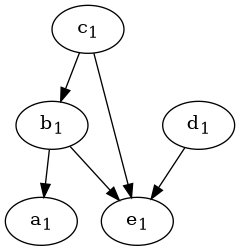
\includegraphics[width=\linewidth,valign=t]{inc/fuzzy_graph_theory/fuzzy_graph_morphism_G1.png}
			\caption{$G_1$.}
		\end{subfigure}
		\quad
		\begin{subfigure}[t]{0.19\textwidth}
			\centering
			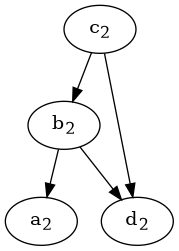
\includegraphics[width=\linewidth,valign=t]{inc/fuzzy_graph_theory/fuzzy_graph_morphism_G2.png}
			\caption{$G_2$.}
		\end{subfigure}
		\caption{Example graphs $G_1$ (left) and $G_2$ (right).}
	\end{figure}
\end{frame}

\begin{frame}
	\frametitle{Interal Representation of Fuzzy Graph Morphisms}

	\begin{figure}[htbp]
		\centering
		\begin{subfigure}[t]{0.20\textwidth}
			\centering
			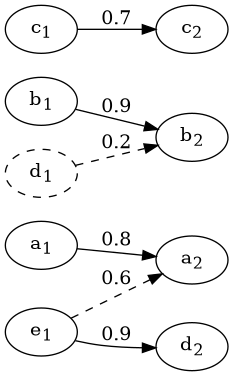
\includegraphics[width=\linewidth,valign=t]{inc/fuzzy_graph_theory/fuzzy_graph_morphism_internal_rho_sigma.png}
			\caption{Vertex morphism $\rho_{\sigma}$.}
		\end{subfigure}
		\quad
		\begin{subfigure}[t]{0.40\textwidth}
			\centering
			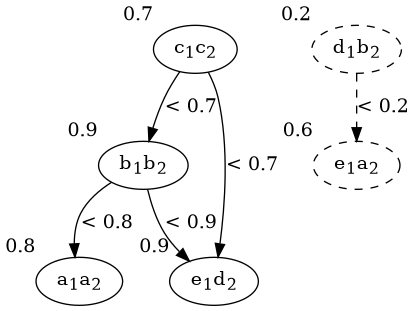
\includegraphics[width=\linewidth,valign=t]{inc/fuzzy_graph_theory/fuzzy_graph_morphism_internal_rho_mu.png}
			\caption{Edge morphism $\rho_{\mu}$.}
		\end{subfigure}
		\quad
		\begin{subfigure}[t]{0.18\textwidth}
			\begin{subfigure}[t]{\textwidth}
				\centering
				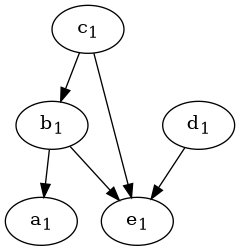
\includegraphics[width=\linewidth,valign=t]{inc/fuzzy_graph_theory/fuzzy_graph_morphism_G1.png}
				\caption{$G_1$.}
			\end{subfigure}
			\begin{subfigure}[t]{0.8\textwidth}
				\centering
				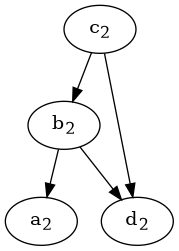
\includegraphics[width=\linewidth,valign=t]{inc/fuzzy_graph_theory/fuzzy_graph_morphism_G2.png}
				\caption{$G_2$.}
			\end{subfigure}
		\end{subfigure}
		\caption{Interal representation of fuzzy graph morphism $\rho(\sigma, \mu)$.}
	\end{figure}
\end{frame}

\begin{frame}
	\frametitle{External Representation of Fuzzy Graph Morphisms}

	\begin{figure}[htbp]
		\centering
		\begin{subfigure}[t]{0.20\textwidth}
			\centering
			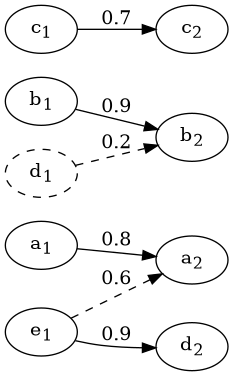
\includegraphics[width=\linewidth,valign=t]{inc/fuzzy_graph_theory/fuzzy_graph_morphism_external_rho_sigma.png}
			\caption{Vertex morphism $\rho_{\sigma}$.}
		\end{subfigure}
		\quad
		\begin{subfigure}[t]{0.20\textwidth}
			\centering
			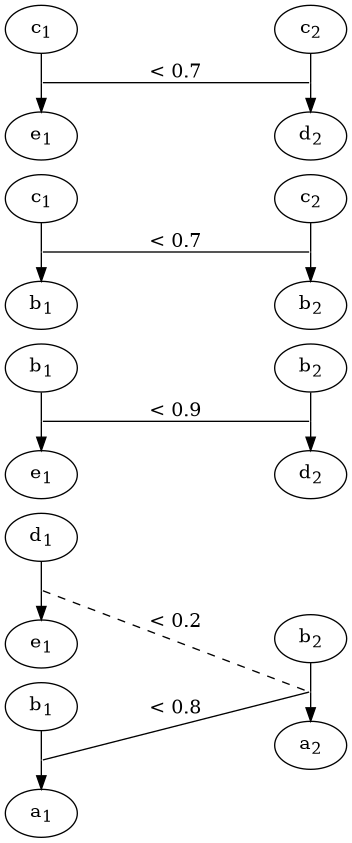
\includegraphics[width=\linewidth,valign=t]{inc/fuzzy_graph_theory/fuzzy_graph_morphism_external_rho_mu.png}
			\caption{Edge morphism $\rho_{\mu}$.}
		\end{subfigure}
		\quad
		\begin{subfigure}[t]{0.18\textwidth}
			\begin{subfigure}[t]{\textwidth}
				\centering
				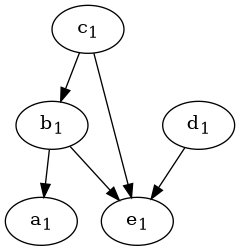
\includegraphics[width=\linewidth,valign=t]{inc/fuzzy_graph_theory/fuzzy_graph_morphism_G1.png}
				\caption{$G_1$.}
			\end{subfigure}
			\begin{subfigure}[t]{0.8\textwidth}
				\centering
				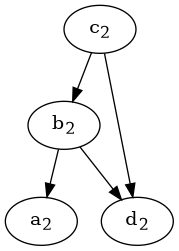
\includegraphics[width=\linewidth,valign=t]{inc/fuzzy_graph_theory/fuzzy_graph_morphism_G2.png}
				\caption{$G_2$.}
			\end{subfigure}
		\end{subfigure}
		\caption{External representation of fuzzy graph morphism $\rho(\sigma, \mu)$.}
	\end{figure}
\end{frame}
